\label{sec:impl}
\Tool's static analysis contains two components. The first takes in Rails source code and generates
a database-aware program dependency graph for every action,\footnote{An action is a member method of a
Ruby controller class. When a web application receives a request, a corresponding action will execute to respond to the request.}
which we refer to as the action
dependency graph (ADG). The second component takes in the ADG, identifies
performance anti-patterns, and synthesizes fixes. We anticipate extending \Tool to tackle other ORM-related performance issues in the future.


%\shan{1.should put much more details here. I have no idea how your tool is implemented. You should save space from describing patterns and put more text here; 2. you didn't explain how fix-suggestion is generated}

\subsection{Database-aware Static Analysis Framework} 
\Tool's static analysis framework goes through the following steps to generate ADG from Ruby on Rails source code.

\textbf{Pre-processing.} \Tool performs inter-procedural analysis on the source code by statically inlining all function calls. It also inlines callbacks such as {\tt ActiveRecord} validations invoked by this action. Since Ruby is dynamically typed, \Tool performs type inference~\cite{furr2009static} to statically determine variable types.

%\Tool first inlines function calls to enable inter-procedural analysis. This
%process involves type inference~\cite{furr2009static}, as Ruby is dynamically typed, 
%and identifying Ruby code that is implicitly
%invoked by an controller action through view rendering, 
%Rails callback functions, {\tt ActiveRecord} validation functions, etc. 

%\alvin{too much detail?}


\textbf{Program dependency graph (PDG) generation.}
\Tool generates a PDG for every controller action, which is the entry function that eventually produces a webpage.   
It uses JRuby 
%\cite{jruby} 
to parse the pre-processed source code, and then builds the PDG from JRuby's intermediate
representation (IR) as this IR nicely captures high-level Ruby semantics via instructions and operands.
As illustrated in Figure \ref{fig:loopinv}b, every node $n$ in the PDG represents a statement in the JRuby IR. 
%and
%is of the type, Assign, Call, Branch, Const, Copy, HashField, ReceiveArg, or
%Return. 
%Related information like source code location and variable names are also kept. 
Every edge $e$ in PDG represents either control dependency or data dependency.
A data-dependency
edge $n_1 \rightarrow n_2$ indicates that the output object $o$ of $n_1$ is used by $n_2$ without
other statements overwriting $o$ in between.

\textbf{Database-aware ADG Generation.}
\Tool then enhances the PDG generated above in three ways to create the ADG: 
(1) changing and splitting some nodes to become 
Query nodes; (2) annotating every Query node with the database table and fields that are read or written; 
(3) annotating every outgoing data-dependency edge of a Query node with the exact field(s) that are used.

To accomplish this, \Tool first analyzes every model class that extends the Rails
{\tt ActiveRecord} interface to determine all the database
tables in the application and the association relationship among them.
For example, analyzing the model classes illustrated in 
Figure~\ref{fig:schema}, \Tool identifies the {\tt users} table
corresponding to the {\tt User} class and similarly for the {\tt Blog} class, and that these two models have 
a one-to-many relationship, i.e., each instance of {\tt User} may own multiple instances of {\tt Blog}.
Second, \Tool analyzes the {\tt schema.rb} file to determine
how many fields each table contains. For example, parsing the
{\tt schema.rb} snippet in Figure~\ref{fig:schema}, \Tool infers the schemas of the {\tt users} and {\tt blogs} tables as
shown in the bottom of the figure.

Third, \Tool identifies queries from three sources: (1) explicit 
invocations of
Rails {\tt ActiveRecord} Query APIs, such as {\tt exist?},
{\tt reload}, {\tt update}, {\tt destroy}, etc;
(2) implicit queries generated by Rails to access object fields, e.g., {\tt $o_1$.$o_2$}, where 
the class of $o_1$ and the class of $o_2$ are associated model classes
(e.g., {\tt user.blogs} would incur a query to
retrieve records in {\tt blogs} table that are associated with
the specific {\tt user} record in {\tt users} table);
(3) embedded SQL queries through {\tt Base.connection.execute}.
%\junwen{it's also thru the ActiveRecord API, similar as the first type}
Any query identified above is represented as a Query node in the ADG.\footnote{At run time,
multiple such queries could be composed by ORM into one SQL query.
Such query chaining does not affect \Tool's analysis.} 
%\alvin{still think that there is too much detail here}
%\junwen{schema helps us differentiate between the fields and the associations, if it only retrieves certain field, then it will not issue a query, but if it retrieve the association, then it will issue a query}


\begin{figure}
    \centering
    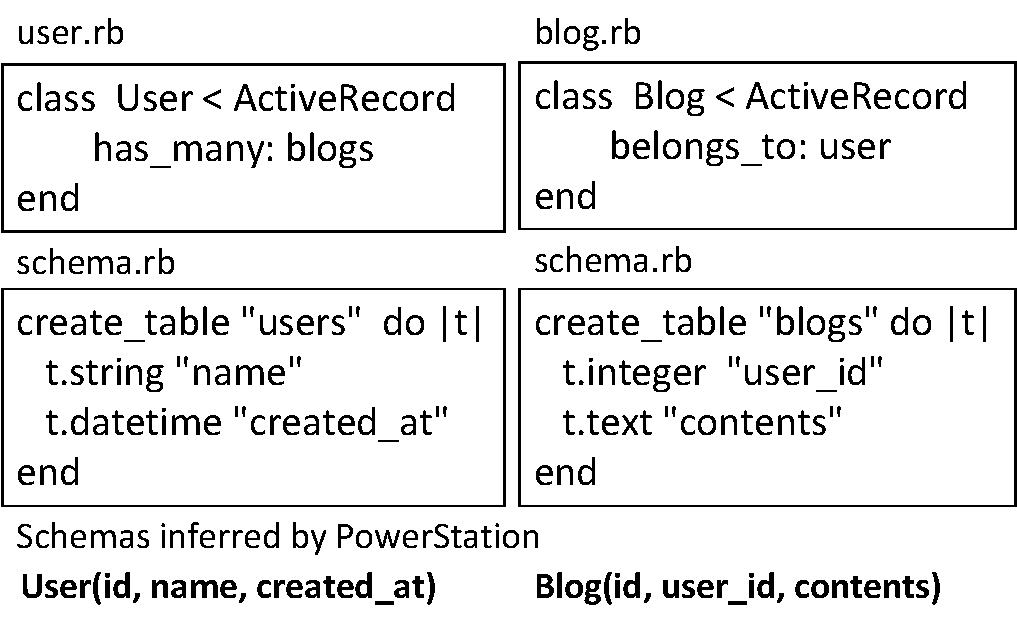
\includegraphics[width=0.7\columnwidth]{figs/schema.pdf}
    \caption{Analyzing table schemas}
    \label{fig:schema}
\end{figure}

\iffalse
\textbf{Final ADG output.} It  is the same as the traditional PDG. Given an action, the ADG of it g is represented as a four-tuple element, g = (V, E, $\mu$, $\delta$), in which, 

\begin{itemize}
\item V contains the vertex which represents the program statement in the action including the involved variables. Moreover, each vertex also contains the corresponding location in the source code including the filename and the line number. 

\item E is the set of edges which represent the dependency between vertices.

\item $\mu$ assigns Assign, Call, Branch, Const, Copy, HashField, ReceiveArg, or Return types to vertices. 

\item $\delta$ assigns whether a edge is Control or Data.
\end{itemize}
Given a source vertex v$_s$, and a target vertex v$_t$, if  v$_s$ is a Branch, and its truth controls
the execution of  v$_t$, then the edge between v$_s$ and v$_t$ is a Control edge. If v$_t$ reads the variable assigns in v$_s$ and there is a execution path between v$_s$ and v$_t$, then the edge is a Data edge.
\fi

\subsection{Detecting and Fixing Anti-patterns}
\textbf{Loop invariant queries.} \Tool first identifies all query nodes inside loop bodies in ADG. For each such node $n$, 
it checks the incoming data-dependency edges of $n$. If all of these edges start from outside the loop $L$
where $n$ is located, then $n$ is identified as a loop-invariant query, such as ``Call: v3...'' in Figure \ref{fig:loopinv}b.
%The analysis will output the query statement as well as the filename and line number as the location information, and  the location of the start of the loop. %If this statement has not been assigned to the local variable inside the loop, we will also generate a variable name  randomly in order to avoid the name conflict with other variables. 
To fix this, \Tool inserts a new Assign statement before the start of the loop, where a newly created variable $v$
gets the return value of the loop-invariant query, and replaces every invocation of the loop-invariant query inside loop $L$
with $v$.

\textbf{Dead store queries.}  \Tool checks every ADG node that issues a reload query, i.e., {\tt o.reload}, %\alvin{does it have to assign to the same object?} 
and checks its out-going data-dependency
edge. If there is no such edge, i.e., the reloaded content is not used, then the query is marked as a dead-store query that is deleted by \Tool.
%To synthesize a fix, \Tool simply deletes the reload statement.

\textbf{Unused data retrieval queries.} For every Read query node $n$ in the ADG, \Tool first computes the database fields loaded by $n$ that are used subsequently. This is the union of
the \textit{used fields} associated with every out-going data-dependency edge of $n$. 
\Tool then checks if every loaded field is used. For every unused field,
\Tool either deletes $n$, if none of the fields retrieved by $n$ are used, or adds field
selection {\tt .select(:f1, :f2, \ldots)} to the original query in $n$ so that only used fields
{\tt f1}, {\tt f2} are loaded. 


\textbf{Common sub-expression queries.} \Tool checks every query node $q_0$
in ADG to see if $q_0$ has out-going data-dependency edges
to at least two query nodes $q_1$ and $q_2$ in the same control path. If that is the case, then
by default, Rails would issue at least two SQL queries that
share common sub-expression $q_0$ at 
run time, one composing $q_0$ and $q_1$ and one composing 
$q_0$ and $q_2$,
%\shan{Don't you need to check if $q_1$ and $q_2$ might appear in one control path?}
with the latter unnecessarily evaluates $q_0$ again.
%As mentioned, query components are composed through call chains \cong{make sure it is discussed}. It is often seen that a partial chain diverges into multiple chains later, as a result, the component in the partial chain is shared by different queries. For example, {\tt u=user.where(:age>21)} is a partial chain that selects users over 21 years old. The application later gets the count of such users and a list of blogs written by them by calling {\tt u.count} and {\tt u.blogs}, which correspond to a {\tt COUNT} query and a {\tt JOIN} query. These two queries share the same subexpression {\tt `WHERE age>21`}. Powerstation finds common subexpression by discovering the above pattern: if a partial call chain contains any query vertex, and is later diverged into multiple chains where multiple queries are issued, then these queries share common subexpression.\shan{???}
This can be optimized by changing the query plan and caching the common intermediate result for reuse~\cite{yan:cikm17}. 
Doing so requires issuing raw SQL commands that are currently not supported
by Rails {\tt ActiveRecord} APIs. 
%Since such fix might hurt code readability, the current prototype of \Tool does not automatically
%generate such fixes. \alvin{is the current goal of \Tool to generate `human readable' code? I see \Tool as a compiler like gcc and hence does it matter how ugly the generated code looks like?} \junwen{PowerStation now makes change on source code, so the goal is to generate human readable code}

%We chain the query vertex in ADG through the data edge and check whether the same query function is used in two different query function chains\shan{Don't understand this sentence}. If so, the corresponding queries share a common subexpression\shan{Don't understand. What is the common sub-expression?}.
%Fixing this problem requires operation to the database such as creating a template, unfortunately, Rails doesn't provide such API for us to automatically solve it in the source code\shan{Doesn't Ruby allows you to embed raw SQL command in program? Why cannot you do that?}.

\textbf{API Misuses.} 
\Tool uses regular expression matching to find inefficient API misuses as in previous work~\cite{junwen:icse2018}.
%\shan{Do you do this on ADG or not? Your current description does not sound like so}. \junwen{both are implemented, since regex is easier to describe, so I chose it.}
Since these API mis-use patterns are simple, \Tool also synthesizes patches for each API mis-use pattern through regular expressions. %\alvin{do all misues only involve one function call as in the case of `count'? If not what if instead of writing o.f1.f2 they wrote v = o.f1; v.f2 ?}


\textbf{Inefficient rendering.} \Tool checks every loop in the ADG to see if it iterates through objects returned by queries and contains a Rails view helper function 
such as {\tt link\_to} in every loop iteration.
If so, \Tool identifies the code as having the inefficient rendering
problem. To fix this, \Tool  
%\alvin{why suggest? does it not do it automatically?} 
hoists the helper function out of the loop, assigns its result to a newly created variable, and replaces the original
helper function in the loop with {\tt gsub} (a string substitution function) on the newly created variable, as shown in Figure \ref{fig:rendering}. Doing so removes the redundant rendering that is performed on every loop iteration in the original code.

\begin{figure}
    \centering
    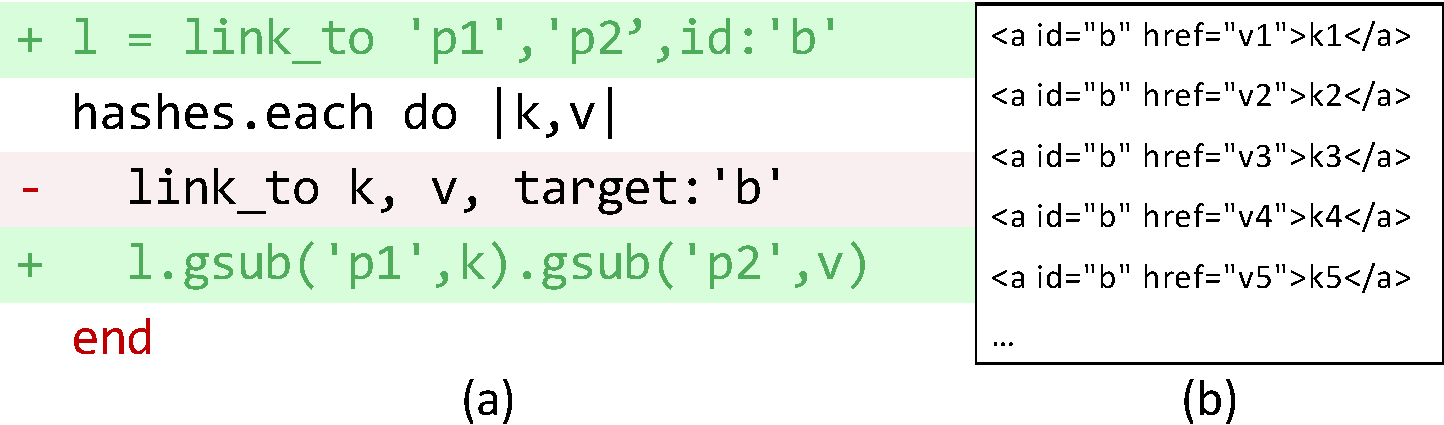
\includegraphics[width=0.7\columnwidth]{figs/rendering.pdf}
% \vspace{-0.1in}
    \caption{Fix for inefficient rendering %{\tt content\_tag (:div, value} creates a xxxx)
    \textmd{({\tt gsub} is a string substitution API, replacing its first parameter with the second)}
    }
    \label{fig:rendering}
%    \small{The {\tt content\_tag(:div, value)} will create a div tag as {\tt <div>value</div>}.}

\end{figure}

\textbf{Discussion.}
%\Tool static analysis could report false positives. Because the analysis is targeted on single action. 
Like other code refactoring tools, \Tool currently suggests fixes to the user rather than deploying them automatically. This is important for Dead Store and Unused Data cases, since the \Tool-suggested fixes would change application semantics if the retrieved data is used in multiple actions.
%make \Tool fixes invalid---developers can check before accepting \Tool fixes. 
For the other cases, however, \Tool's suggested fixes do preserve program semantics.